\documentclass[12pt]{article}
\usepackage[hidelinks]{hyperref}    
\usepackage[all]{hypcap}
\usepackage{xcolor}
\usepackage{amsmath}
\usepackage{graphicx}
\graphicspath{{../_images/}}
\definecolor{goldenrod_yellow}{RGB}{218, 165, 32}
\definecolor{dark_green}{RGB}{116, 148, 121}
\definecolor{exists_pink}{RGB}{255, 132, 212}
\title{\textbf{Logica per l'informatica\\Brutta}}
\date{15 ottobre 2024}
\author{Andrea Malvezzi}
\begin{document}
\maketitle
\pagebreak
\tableofcontents
\pagebreak
\section{esempio albero spiegato}
parto con:
\begin{equation}
    B, D \wedge A \vdash A \wedge (B \Rightarrow C) \Rightarrow C \label{es:exp:albero_deduzione_naturale}
\end{equation}
Ciò che è prima del $\vdash$ si dice gamma ($\gamma$) e contiene le ipotesi globali (senza quadre nell'albero), mentre ciò che viene dopo si dice radice ($F$). Si dice $\gamma \vdash F$, da gamma derivo $F$.\\
\begin{figure}[!htb]
    \centering
    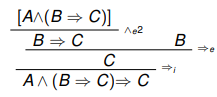
\includegraphics[width=.9\linewidth,height=.40\textheight,keepaspectratio]{brutta/albero_deduzione.png} % essenzialmente resiza l'immagine
    \begin{center}
        \caption{\label{fig:no_iniett_example}Esempio di albero di deduzione naturale.} % label fuori da caption spesso non va, mettilo dentro
    \end{center}
\end{figure}\\
Qui opto per una lettura top-down e parto da ciò che devo dimostrare per ridurmi a dimostrare altro. Parto dal dimostrare $[A \wedge (B \Rightarrow C)]$, applico la regola (?) dell'and, dimostro $B \Rightarrow C$. Ma dalle ipotesi globali (quelle in $\gamma$) ho $B$, perciò $C$ (tramite la regola (?)) e quindi per finire, applicando la regola (?) dimostro la radice $F$.
\pagebreak
\section{Regole}
Nella figura seguente $F_n$ sono dette premesse della regola da applicare, mentre $F$ si dice conclusione della regola.\\
\begin{figure}[!htb]
    \centering
    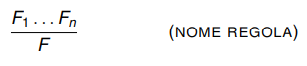
\includegraphics[width=.9\linewidth,height=.40\textheight,keepaspectratio]{brutta/regole_albero.png} % essenzialmente resiza l'immagine
    \begin{center}
        \caption{\label{fig:regole_albero}Esempio di albero con n regole e una conclusione (ovviamente).} % label fuori da caption spesso non va, mettilo dentro
    \end{center}
\end{figure}\\
Una regola senza premesse si dice assiome (ma è diverso da quelli della logica del primo ordine).
\section{Costruire un albero}
Un albero si deve costruire componendo ricorsivamente le regole di inferenza. Nella figura seguente, $F_n$ sono le regole di $H_1$, mentre $G_n$ sono le regole di $H_l$, dove $F_n$ su $H_1$ è un sottoalbero di induzione naturale.
\begin{figure}[!htb]
    \centering
    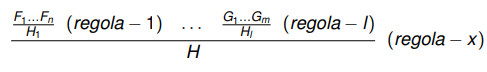
\includegraphics[width=.9\linewidth,height=.40\textheight,keepaspectratio]{brutta/costruzione_ricorsiva.png} % essenzialmente resiza l'immagine
    \begin{center}
        \caption{\label{fig:albero_ricorsivamente}Costruzione di un albero tramite composizione ricorsiva delle regole di inferenza.} % label fuori da caption spesso non va, mettilo dentro
    \end{center}
\end{figure}
\pagebreak
\section{Correttezza di un albero}
Se una premessa contempla ipotesi scaricate, esse vanno integrate tramite applicazioni nella formula finale. 
\begin{figure}[!htb]
    \centering
    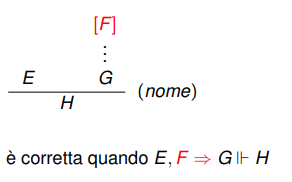
\includegraphics[width=.9\linewidth,height=.40\textheight,keepaspectratio]{brutta/ipotesi_globali_formula_finale.png} % essenzialmente resiza l'immagine
    \begin{center}
        \caption{\label{fig:correttezza_albero}Esempio di albero costruito correttamente.} % label fuori da caption spesso non va, mettilo dentro
    \end{center}
\end{figure}
\section{Invertibilità di una regola}
Una regola è invertibile quando la sua conclusione implica le ipotesi, ergo quando c'é coimplicazione tra conclusione e premesse.\\
L'invertibilità è importante perché permette di ragionare top-down senza entrare in un vicolo cieco da cui non si può fare backtracking.\\
Vedi esempio sui LUCIDI.
\section{AND}
Regola di introduzione ($\wedge_i$):
\begin{equation}
    \dfrac{F_1 \text{ } F_2}{F_1 \wedge F_2}
\end{equation}
Lettura bottom-up: se $F_1$ e $F_2$ allora $F_1 \wedge F_2$.\\
Lettura top-down: per dimostrare $F_1 \wedge F_2$ debbo dimostrare sia $F_1$ che $F_2$.\\
Notare come questa \textbf{regola suoni bene} in italiano: GENERALMENTE (non è una regola ma solo un'osservazione) le regole che suonano bene in italiano sono invertibili.\\
Regola di eliminazione ($\wedge_e$):
\begin{figure}[!htb]
    \centering
    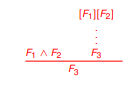
\includegraphics[width=.9\linewidth,height=.40\textheight,keepaspectratio]{brutta/eliminazione_and.png} % essenzialmente resiza l'immagine
    \begin{center}
        \caption{\label{fig:eliminazione_and}Regola di eliminazione dell'and.} % label fuori da caption spesso non va, mettilo dentro
    \end{center}
\end{figure}\\
\begin{figure}[!htb]
    \centering
    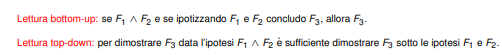
\includegraphics[width=.9\linewidth,height=.40\textheight,keepaspectratio]{brutta/letture_eliminazione_and.png} % essenzialmente resiza l'immagine
    \begin{center}
        \caption{\label{fig:lettura_eliminazione_and}Letture regola di eliminazione dell'and.} % label fuori da caption spesso non va, mettilo dentro
    \end{center}
\end{figure}\\
\begin{figure}[!htb]
    \centering
    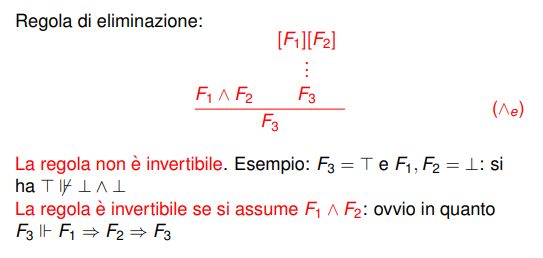
\includegraphics[width=.9\linewidth,height=.40\textheight,keepaspectratio]{brutta/non_sempre_invertibile_eliminazione_and.png} % essenzialmente resiza l'immagine
    \begin{center}
        \caption{\label{fig:non_sempre_inv_eliminazione_and}La regola è invertibile solo supponendo che $F_1 \wedge F_2$, perché sasrebbe impossibile dimostrare che questo è falso partendo da top ($F_3$).} % label fuori da caption spesso non va, mettilo dentro
    \end{center}
\end{figure}\\
Importante dare sempre precedenza alle regole che splittano (eliminazione in questo caso dell'and). La and introduzione apre due sottodimostrazioni da fare entrambe, mentre la and eliminazione ne apre sempre due MA una è generalmente già dimostrata per le ipotesi locali.\\
Ci sono altre due regole alternative di eliminazione (le più popolari su internet):
\begin{equation}
    \dfrac{F_1 \wedge F_2}{F_1}, (\wedge_{e_1})
\end{equation}
\begin{equation}
    \dfrac{F_1 \wedge F_2}{F_2}, (\wedge_{e_2})
\end{equation}
Che non sono invertibili.
\pagebreak
\subsection{Riassuntino}
eliminazione $\rightarrow$ spezzo l'ipotesi iniziale (avendo $(A \wedge B) \wedge (C \wedge D)$ ottengo [$A \wedge B$] [$C \wedge D$]) e mano a mano spezzo sempre di più.\\
introduzione $\rightarrow$ semplifica la conclusione della regola nelle componenti che la compongono.\\
eliminazione 1 e 2 son più un risalire a una delle variabili globali, come accadeva nell'eliminazione, ma stavolta esplicitando il ragionamento.\\
VEDI ESEMPI ALBERI SUI LUCIDI PER CAPIRE BENE. 
\section{OR}
Regole di introduzione:
\begin{equation}
    \dfrac{F_1}{F_1 \vee F_2}, (\vee_{i_1})
\end{equation}
\begin{equation}
    \dfrac{F_2}{F_1 \vee F_2}, (\vee_{i_2})
\end{equation}
Non sono invertibili. Prima si opta per quella di eliminazione, ovvero:
\begin{figure}[!htb]
    \centering
    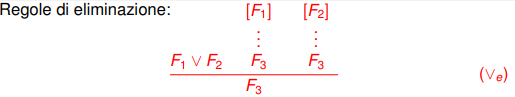
\includegraphics[width=.9\linewidth,height=.40\textheight,keepaspectratio]{brutta/eliminazione_or.png} % essenzialmente resiza l'immagine
    \begin{center}
        \caption{\label{fig:eliminazione_or}Non invertibile: $F_3 = \top$ e $F_1 = F_2 = \bot$. Quando posso dimostrare $F_1 \vee F_2$, allora si può invertire.} % label fuori da caption spesso non va, mettilo dentro
    \end{center}
\end{figure}\\
\end{document}